\documentclass[12pt]{article}

\title{On the Monte Carlo simulation of anisotropic Newtonian gravitation}
\author{S. Halayka\footnote{sjhalayka@gmail.com}}
\date{\today\;\currenttime}

\usepackage{datetime}
\usepackage{listings}
\usepackage{cite}
\usepackage{xcolor}
\usepackage{graphicx}
\usepackage{setspace}
\usepackage{amsmath}
\usepackage{url}
\usepackage[margin=0.8in]{geometry}
\usepackage{listings}


\usepackage{xcolor}
\lstset { %
    language=C++,
    backgroundcolor=\color{black!5}, % set backgroundcolor
    basicstyle=\footnotesize,% basic font setting
    showstringspaces=false,
}


%\doublespace

%\usepackage[]{lineno}
%\linenumbers


\begin{document}



 
\maketitle

\begin{abstract}
This paper contains a short introduction to anisotropic Newtonian gravitation.
The main focus is on some C++ code.
\end{abstract}



\section{Introduction}

\begin{equation}
\alpha = \frac{\beta(R + \epsilon) - \beta(R)}{\epsilon}.
\end{equation}

\begin{equation}
g = \frac{-\alpha}{r^2}. 
\end{equation}

\begin{equation}
a_N = \sqrt{\frac{n G c \hbar \log 2}{4 k \pi R^4}},
\end{equation}
\begin{equation}
v_N = \sqrt{a_N R}.
\end{equation}

\begin{equation}
v_{\textrm{flat}} = x v_N
\end{equation}
where $x = 2$ for example.
\begin{equation}
a_{\textrm{flat}} = \frac{v_{\textrm{flat}}^2}{R} = \frac{g R c \hbar \log 2}{k 2 \pi M}.
\end{equation}
\begin{equation}
g_N = \frac{a_N k 2 \pi M}{R c \hbar \log 2}. 
\end{equation}



\begin{equation}
a_{\textrm{flat}} \propto g.
\end{equation}
\begin{equation}
a_{\textrm{ratio}} = \frac{a_{\textrm{flat}}}{a_N}. 
\end{equation}
\begin{equation}
g_{\textrm{ratio}} = \frac{g}{g_N}. 
\end{equation}

$D$ is where $g_{\textrm{ratio}} \geq a_{\textrm{ratio}}$.



\begin{figure} 
\centering
\label{fig3}
  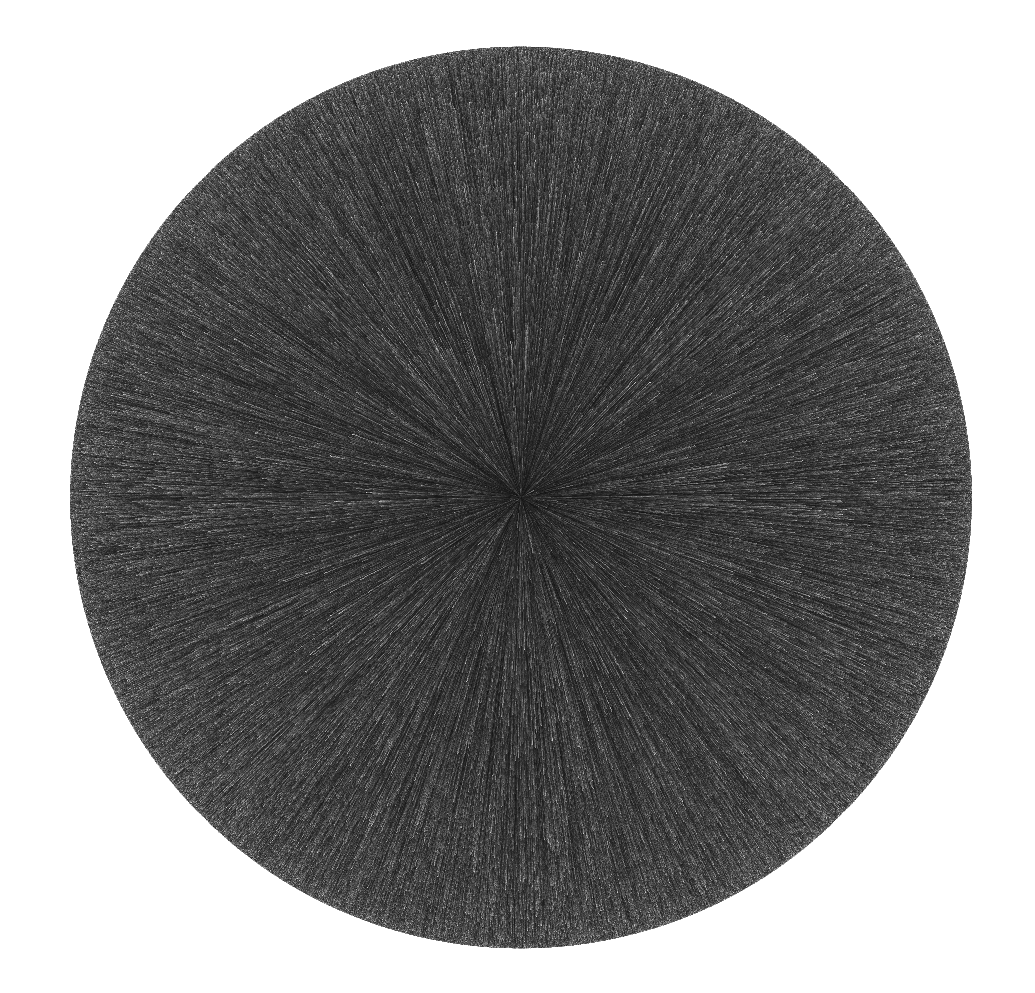
\includegraphics[width = 1.5 in]{3.png}
  \caption{
Where $D = 3$, as viewed from the side.
The field lines are isotropic, spherical.
}
\end{figure}
\begin{figure} 
\centering
\label{fig4}
  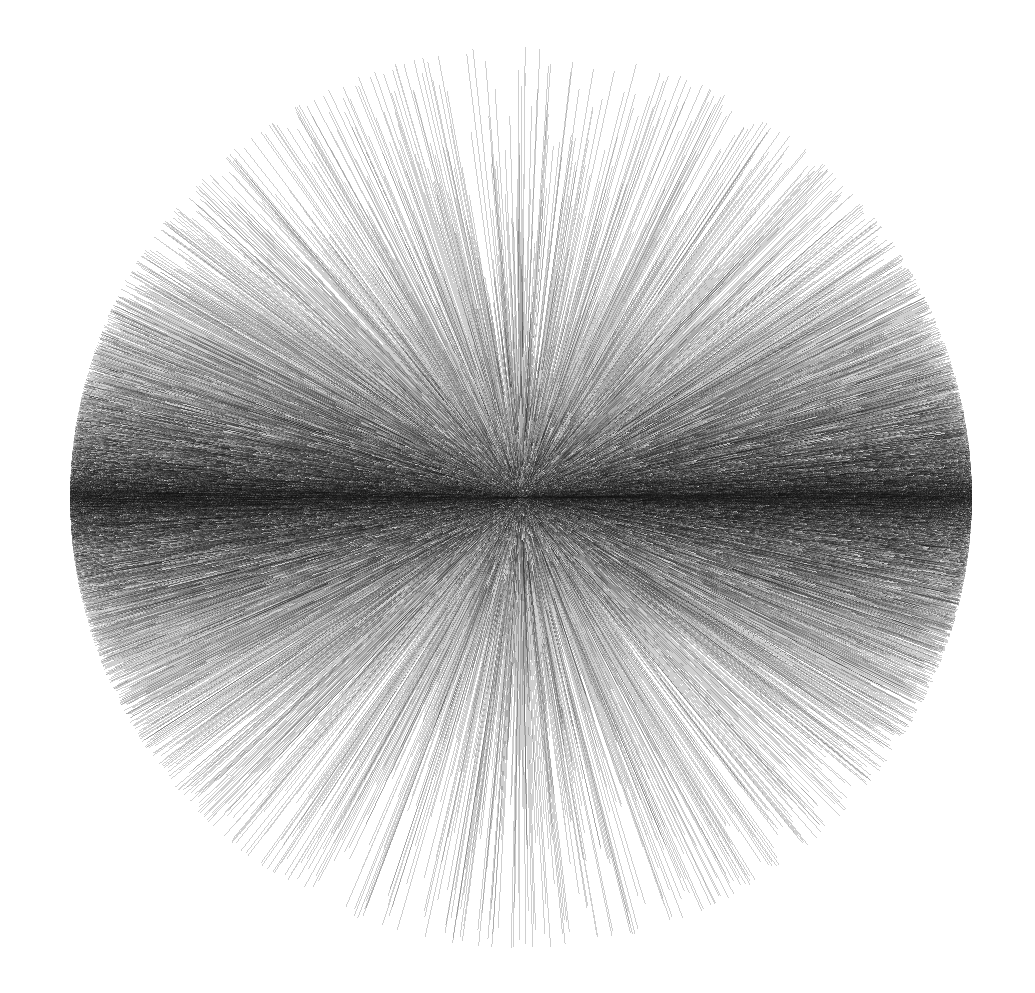
\includegraphics[width = 1.5 in]{2.1.png}
  \caption{
Where $D = 2.1$, as viewed from the side.
The field lines are increasingly anisotropic.
}
\end{figure}
\begin{figure} 
\centering
\label{fig5}
  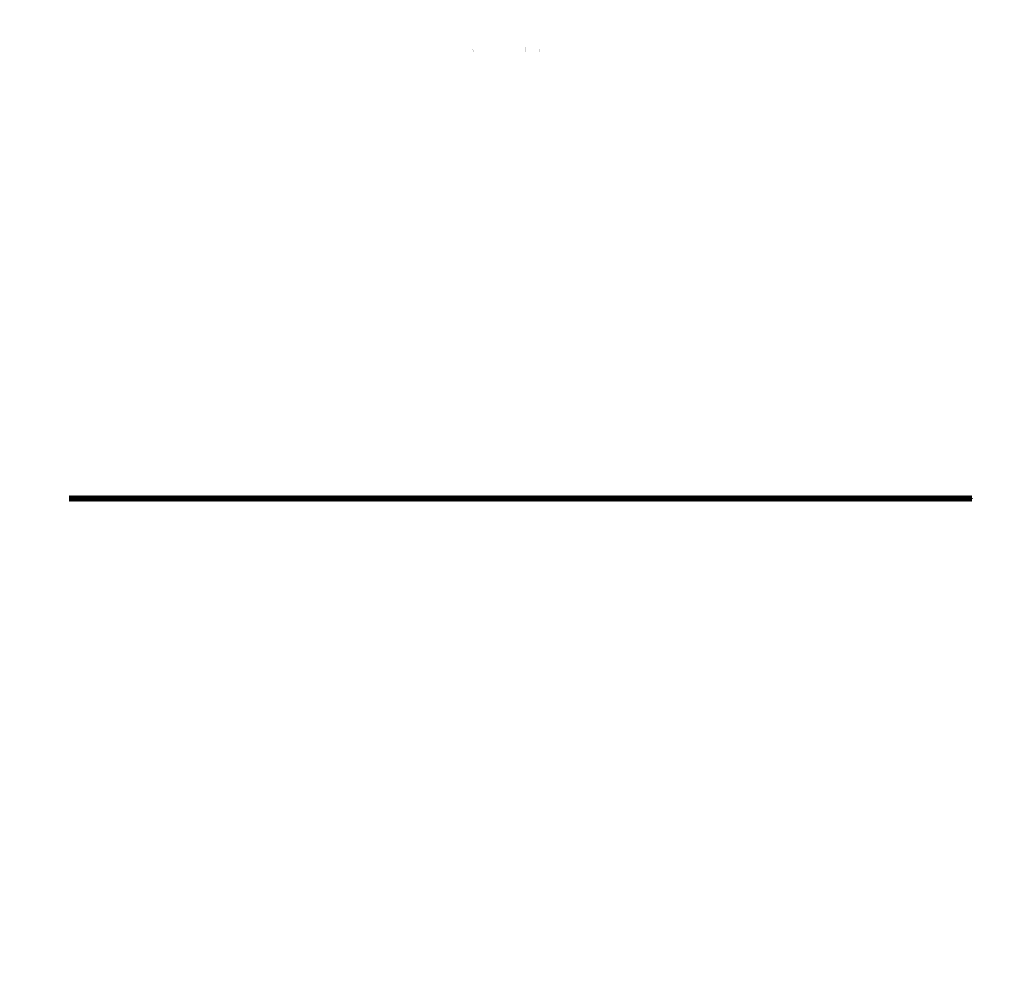
\includegraphics[width = 1.5 in]{2.001.png}
  \caption{
Where $D = 2.001$, as viewed from the side.
The field lines are anisotropic, disk-like.
}
\end{figure}





\begin{figure} 
\centering
\label{fig3}
  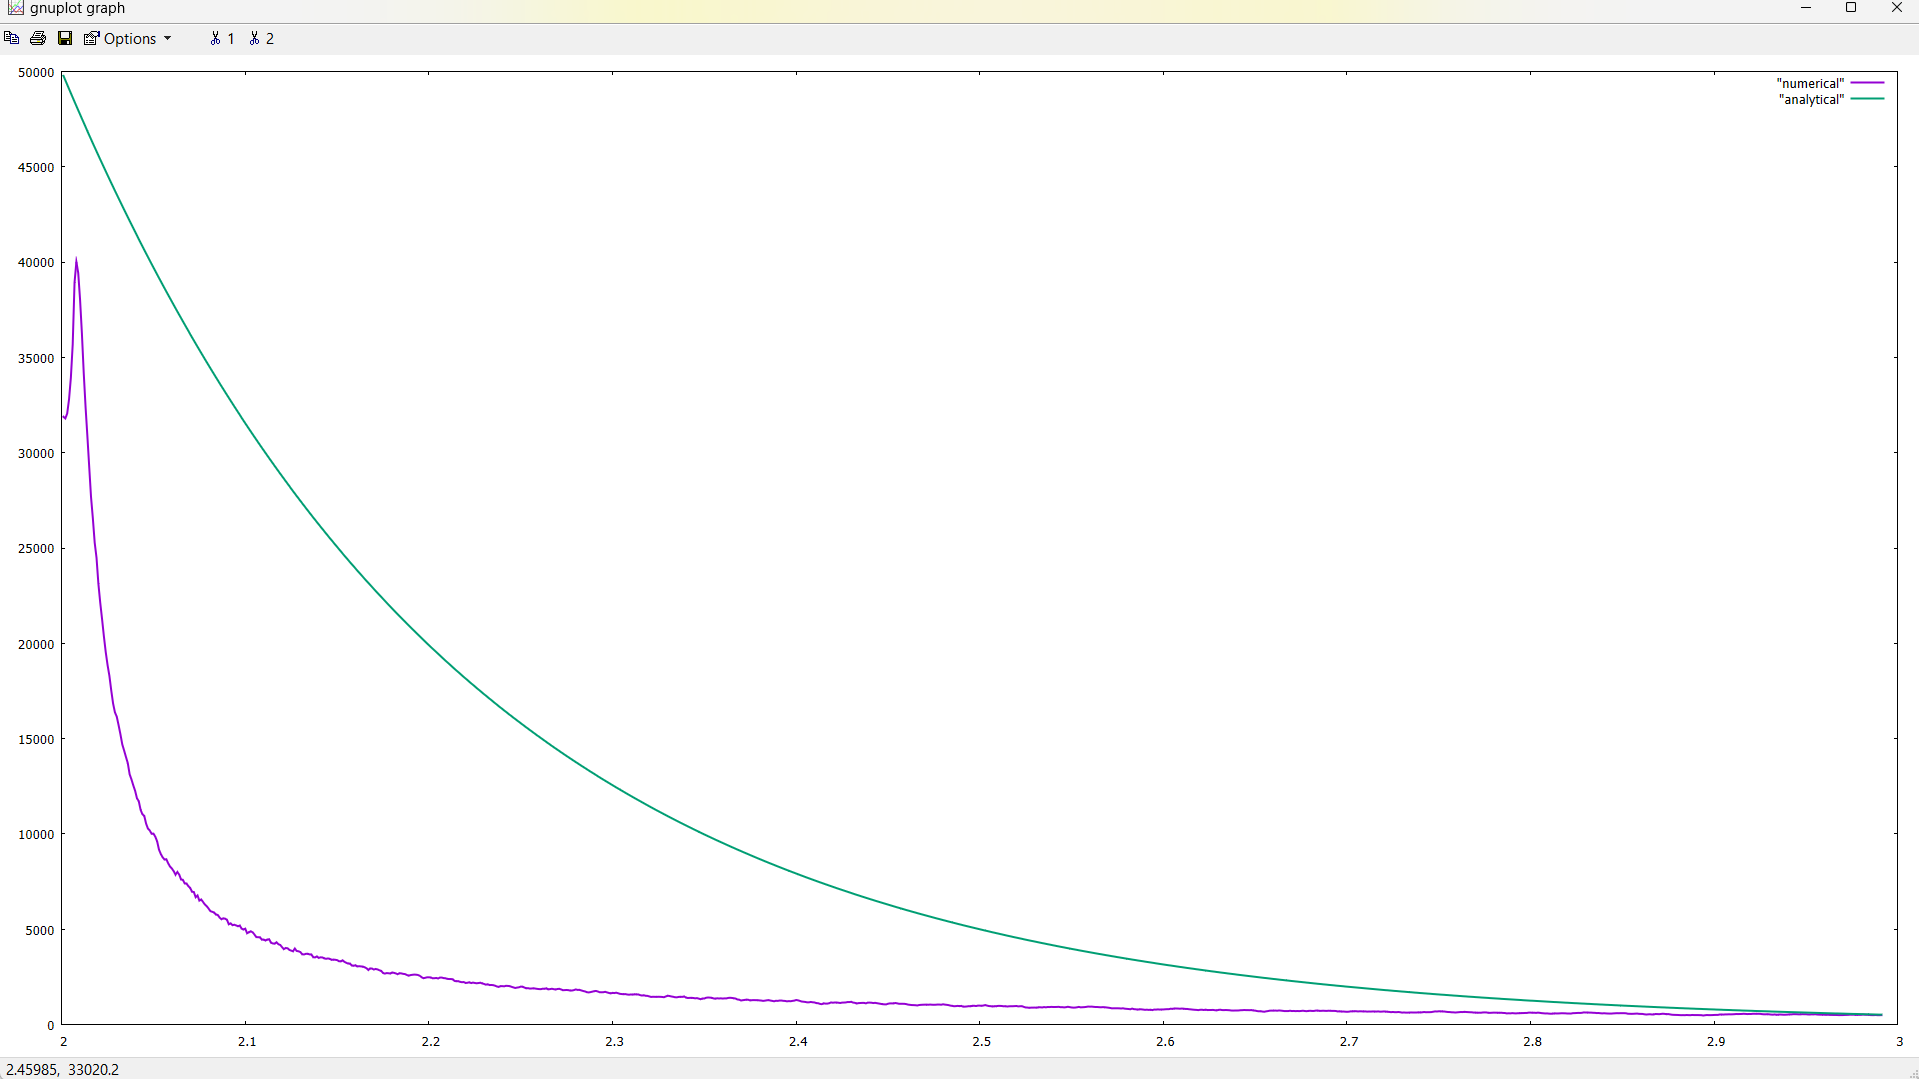
\includegraphics[width = 7 in]{numerical_versus_analytical.png}
  \caption{
$R = 100$, $r = 1$, $n = 10^{8}$, $\epsilon = 1$.
The analytical plot is generated by the formula $y = n / (2 R^D)$.
}
\end{figure}





\begin{thebibliography}{9}

\bibitem{misner} Misner et al. Gravitation. (1970)

\bibitem{hooft} `t Hooft. Dimensional reduction in quantum gravity. (1993)
\bibitem{susskind} Susskind. The World as a Hologram. (1994)




\end{thebibliography}














\end{document}









